\documentclass[conference]{IEEEtran}

% *** GRAPHICS RELATED PACKAGES ***
%
\ifCLASSINFOpdf
   \usepackage[pdftex]{graphicx}
  % declare the path(s) where your graphic files are
  % \graphicspath{{../pdf/}{../jpeg/}}
  % and their extensions so you won't have to specify these with
  % every instance of \includegraphics
  % \DeclareGraphicsExtensions{.pdf,.jpeg,.png}
\else
  % or other class option (dvipsone, dvipdf, if not using dvips). graphicx
  % will default to the driver specified in the system graphics.cfg if no
  % driver is specified.
  % \usepackage[dvips]{graphicx}
  % declare the path(s) where your graphic files are
  % \graphicspath{{../eps/}}
  % and their extensions so you won't have to specify these with
  % every instance of \includegraphics
  % \DeclareGraphicsExtensions{.eps}
\fi

% *** MATH PACKAGES ***
%
\usepackage{amsmath}
\usepackage{mathtools}
\DeclarePairedDelimiter\floor{\lfloor}{\rfloor}


% *** PDF, URL AND HYPERLINK PACKAGES ***
%
%\usepackage{url}


\usepackage[brazilian]{babel}
\usepackage[utf8]{inputenc}
%\usepackage[T1]{fontenc}
\usepackage{fancyhdr}


% correct bad hyphenation here
%\hyphenation{op-tical net-works semi-conduc-tor}


\pagestyle{fancy}
%\fancyhf{}
\chead{VII Workshop de P\'{o}s-Gradua\c{c}\~{a}o - Engenharia de Computa\c{c}\~{a}o - WPGEC 2018}
\renewcommand{\headrulewidth}{2pt}

\pagenumbering{gobble}

\begin{document}

%
% paper title
% Titles are generally capitalized except for words such as a, an, and, as,
% at, but, by, for, in, nor, of, on, or, the, to and up, which are usually
% not capitalized unless they are the first or last word of the title.
% Linebreaks \\ can be used within to get better formatting as desired.
% Do not put math or special symbols in the title.
\title{Diagnóstico do Glaucoma a partir de imagens de OCT e Redes Neurais Profundas (DNN)}



% conference papers do not typically use \thanks and this command
% is locked out in conference mode. If really needed, such as for
% the acknowledgment of grants, issue a \IEEEoverridecommandlockouts
% after \documentclass

% for over three affiliations, or if they all won't fit within the width
% of the page, use this alternative format:
% 
\author{\IEEEauthorblockN{BRAGA, S. J.\IEEEauthorrefmark{1};
GOMI, E. S.\IEEEauthorrefmark{1}}
\IEEEauthorblockA{\IEEEauthorrefmark{1}Escola Politécnica da Universidade de São Paulo}}


% make the title area
\maketitle

\thispagestyle{fancy}

% As a general rule, do not put math, special symbols or citations
% in the abstract
\renewcommand{\abstractname}{Abstract}
\begin{abstract}
Abstract here.
\end{abstract}

\renewcommand\IEEEkeywordsname{Keywords}
\begin{IEEEkeywords}
\label{Keywords}
word 1; word 2.
\end{IEEEkeywords}

\renewcommand{\abstractname}{Resumo}
\begin{abstract}
\label{Resumo}
\'E necess\'aria a inser\c{c}\~{a}o do resumo para artigo escrito em Portugu\^{e}s.
\end{abstract}

\renewcommand\IEEEkeywordsname{Palavras-chave}
\begin{IEEEkeywords}
\label{Palavras-chave}
palavra 1; palavra 2.
\end{IEEEkeywords}

\renewcommand\IEEEkeywordsname{Classifica\c{c}\~{a}o}
\begin{IEEEkeywords}
	\label{classificacao}
	Mestrado
\end{IEEEkeywords}

\renewcommand\IEEEkeywordsname{Categoria}
\begin{IEEEkeywords}
	\label{Categoria}
	Iniciante 
\end{IEEEkeywords}

\IEEEpeerreviewmaketitle


\section{Introdução}

\section{Diagnóstico de glaucoma}

\section{Redes neurais profundas}

  \subsection{Transfer Learning}

  \subsection{Redes pré-treinadas}

\section{Experimentos e resultados}

%setup do servidor, quais gpus
%utilizando caffe
%qual o objetivo dos experimentos, como foi avaliado

Os experimentos foram conduzidos em um servidor com Ubuntu 16.04 com duas GPUs NVidia Quadro K5200 com 8GB de memória cada, 24 CPUs Intel Xeon e 128GB de memória RAM. O framework de deep learning utilizado em todos os experimentos foi o Caffe, fornecido pela universidade de Berkeley \cite{jia2014caffe}.

O objetivo dos experimentos, com e sem transfer learning, é a classificação binária de olhos normais ou com glaucoma em imagens de OCT. A performance das redes foram avaliadas utilizando um conjunto menor de imagens não vistas para classificação e cálculo das métricas de avaliação. O mesmo conjunto de imagens é utilizado em todos os experimentos. O dataset, pré-processamento e resultados são descritos em detalhes nas próximas seções.

  \subsection{Dataset}

  %aumento do dataset, rotações aleatorias entre 0 e 360
  %divisao treino e validação

  O dataset original foi obtido com o departamento de oftalmologia da Unicamp. O dataset consiste de imagens de OCT de 56 olhos com glaucoma e 66 olhos normais, totalizando 122 pacientes. Os gráficos de espessura de fibras nervosas foram obtidos através da extração das imagens do PDF do exame. Foram selecionados para o experimento somente os olhos de pacientes que foram manualmente classificados por especialistas.

  Para a separação do dataset em treino e validação, foram selecionados 20\% de olhos normais e 20\% de olhos com glaucoma para validação, e o restante para treino, totalizando 98 imagens de treino e 24 para validação. As imagens selecionadas para teste não estão presentes no dataset de treino, para que o algoritmo possa classificar imagens ainda não vistas.

  Para evitar overfitting, foi empregada uma técnica para aumentar o número de exemplos a partir das imagens no dataset de treino. Cada imagem foi rotacionada 100 vezes em ângulos aleatórios entre 0 e 360 graus, gerando assim um dataset de treino com 9800 imagens. As imagens de validação não foram rotacionadas.

  \subsection{Pré-processamento}

  % subtração da media
  % areas pretas para zero absoluto

  Para utilização do transfer learning, foi necessário fazer a subtração do pixel médio em todas as imagens do dataset de treino. O valor médio de cada pixel da imagem é calculado sobre todas as imagens do dataset de treino. Essa imagem média é então subtraída de cada imagem do dataset. Dessa forma, todos os pixels de entrada estão na mesma ordem de grandeza, evitando que os gradientes desapareçam ou explodam.

  Onde houveram falhas na aquisição da imagem, gerando áreas escuras, pixels com valores RGB próximos ao preto foram substituídos pelo valor de preto absoluto RGB (0, 0, 0) para que não tenham influência sobre a decisão do classificador.

  \subsection{Resultados com transfer learning}

  %estrategia de learning rate
  %iterações e tempo de processamento
  %grafico da acuracia

  Neste experimento, utilizamos a mesma arquitetura da rede VGG16, apenas alterando a saída da última camada totalmente conectada para duas saídas, correspondente às duas classes a serem classificadas: normal e glaucoma. 
  
  Os pesos pré-treinados foram carregados para inicialização apenas das camadas convolucionais. As três últimas camadas totalmente conectadas foram iniciadas com valores aleatórios devido à diferença de tamanho entre as imagens do dataset Imagenet e as imagens de OCT classificadas nesse experimento. Essa diferença gera quantidades de parâmetros diferentes na saída da última camada convolucional. Sendo assim, as camadas totalmente conectadas foram inicializadas com valores aleatórios de uma distribuição gaussiana com desvio padrão $0.01$.

  O treinamento foi realizado em todas as camadas da rede, utilizando o gradiente descendente estocástico por $5000$ iterações, com mini batches de 15 imagens. A taxa de aprendizagem inicial foi de $0.001$. A cada 1000 iterações a taxa de aprendizagem foi diminuída utilizando a equação \ref{eq:learning_rate}.

  \begin{equation}
    base\_lr * \gamma^{\floor*{\frac{iter}{step}}}
    \label{eq:learning_rate}
  \end{equation}

  Onde $base\_lr$ é a taxa de aprendizagem inicial, $\gamma$ é um parâmetro do Caffe definido com o valor $0.1$, $iter$ é o número da iteração atual e $step$ é um parâmetro definido como $1000$.

  \begin{figure}[!tp]
    \centering
    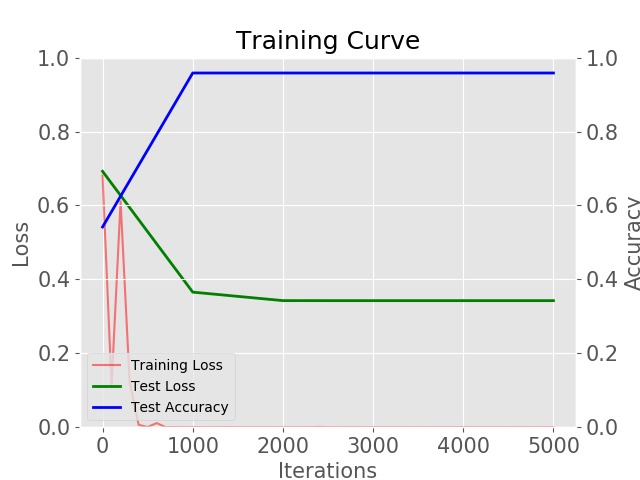
\includegraphics[width=2.5in]{img/curve_vgg16.png}
    \caption{Acurácia e perda de treino e validação da rede VGG16 com transfer learning.}
    \label{fig:acuracia_vgg16_transfer}
  \end{figure}

  \subsection{Resultados sem transfer learning}

  %iterações e tempo de processamento
  %grafico da acuracia

\section{Discussão}

%dificuldades para definir os parametros corretos de treinamento
%dataset pequeno
%tempo de treinamento(?)

\section{Conclusão}



%Use BIB file
\bibliographystyle{abntex2-num}
\bibliography{template}

% that's all folks
\end{document}


